% Chapter Template

\chapter{Two-stage Classification Method for Automatic Reading Comprehension } % Main chapter title

\label{Chapter3} % Change X to a consecutive number; for referencing this chapter elsewhere, use \ref{ChapterX}

\section{Introduction}

Teaching reading comprehension in an online learning environment is very challenging to the instructors as they need to provide the learners with reading material that is authentic, thematically diverse and appropriate to learners' reading level. The system we developed in the previous chapter help language instructors detect the grammatical difficulty of reading materials the find online, but it still does not help eliminate the efforts they need to expend on developing practice exercises and quizzes. In order for second and foreign language learners to master a difficult skill like reading comprehension, they need a lot of practice, which means more training exercises need to be prepared. So in this chapter we design and implement a system that automatically answers comprehension questions given a reading text. While such system still does not fully slove the problem raised, it can signifcantly aid in the automatic creation of reading comprehension practice activities in online learning enviroments. 

Automatic Reading Comprehension is the task of automatically answering comprehension questions based on information derived from short texts. Recently, it has received a special attention from NLP community because of the second release of Stanford Question Answering Dataset (SQuAD 2.0) \citep{rajpurkar2018know}. The dataset consists of 150K questions posed by crowd workers on a set of Wikipedia articles. The answers to these questions lie within the reading passages, though some questions are unanswerable from within the reading passage. What sets SQUAD 2.0 from other data sets is that 50k of its questions are unanswerable, and this requires the learning models not only to find answers, but also to abstain from answering when necessary. \\

The strategy we will use for this task is on two stages \ref{fig:arc-flowchart}. In the first stage, we break the reading passages into sentences, and train a multinomial logisitc regression classifier to find the sentence most likely contains the answer. We also train the classifer to give a null-answer if an answer does not exist. Next, we divide the best candidate sentence from stage one into its consituent phrases, and train another a multinomial logisitc regression classifier to find the consituent phrase that most likely to be the answer to the question. This dual stage method has advantages over other competing models when it comes to speed and consumption of computational resources. 

% The strategy will be used to tackle this task is mainly driven by pure linguistic intuition. Since SQUAD 2.0 task is a question answering task, the answer span lies within one of the given sentences in the paragraph, and then an answer is one of the constituents of the best candidate sentence. Thus, our goal is to, first, find the sentence containing the right answer, and we do by training a logistic regression classifier with some linguistic features. Then, we train another classifier to find the constituent best represent the right answer span within the sentence predicted in the first stage. In order to account for the unanswerability of some of the questions, we add a null-answer as a dedicated class in the first classifier along with the potential sentences. This way, if an answer is not found, the inference process stops without proceeding to the next stage, which saves time and computation. 



\section{Related Work}

There has been a large number of studies that tackle traditional Machine Comprehension tasks, where answers exist within the passage. The difficulty of SQUAD 2.0 task, though, lies in abstaining from answers when no answer span exists in the passage. Thus, in this section we review that models that address this constraint. It worth mentioning that all of the systems described in this section are complicated neural network architectures, and discussing its details is beyond the limitation of this report. 

\citep{DBLP:journals/corr/SeoKFH16} introduced bi-directional attention flow (BiDAF) that uses a recurrent neural network to encode contextual information in both question and passage along with an attention mechanism to align parts of the question to the sentence containing the answer and vise versa. The model offers context representation at multilevel of granularity: character-level, word-level, and contextual embedding. What sets this work from others is that it does not represent the context paragraph into a fixed-length vector. Instead, it dynamically computes vectors at each time step, combines it with the one from the previous layer and allow \textit{flow} through to the next layers. The model outputs confidence scores of start and end index of all potential answers. One problem with this model is that it is not designed to handle unanswerable questions. \citep{DBLP:journals/corr/LevySCZ17} extends the work by assigning a probability to null-answers to account for the questions whose answers do not exist in the corresponding paragraph. It achieves 59.2\% EM score and 62.1\% F1 score.\\

\citep{DBLP:journals/corr/abs-1808-05759} propose a read-then-verify system that can abstain from answering when a question has no answer given the passage. They introduce two auxiliary losses to help the neural reader network focus on answer extraction and no-answer detection respectively, and then utilize an answer verifier to validate the legitimacy of the predicted answer. One essential contribution is answer-verification. The model incorporates a multi-layer transformer decoder to recognize the textual entailment that supports the answer in and passage. This model achieves an ExactMatch EM score of 71.6\% and 74.23\% F1 on SQuAD 2.0. \\

\citep{DBLP:journals/corr/abs-1811-11934} proposes a new hierarchical attention network that mimics the human process of answering reading comprehension tests. It gradually focuses attention on the part of the passage containing the answer to the question. The modal comprises of three layers. a) \textbf{encoder layer}: builds representations to both the question and the passage using a concatenation of word-embedding representation \citep{pennington2014glove} and a pre-trained neural language modal \citep{Peters:2018} b) \textbf{Attention layer}: its function is to capture the relationship between the question and the passage at multiple levels using self-attention mechanisms. c) \textbf{Matching layer}: given refined representation for both question and passage, a bi-linear matching layer detects the best answer span for the question. This method achieves state-of-the-art results as of September 2018. Their single model achieves 79.2\% EM and 86.6\% F1 score, while their ensemble model achieves 82.4\% EM and 88.6\% F1 Score. \\

Current models that have shown significant improvement on Machine Comprehension tasks and other similar ones owe their success to a new neural architecture called transformer networks \citep{DBLP:journals/corr/VaswaniSPUJGKP17}. It has become the \emph{de facto} in recent sequential learning tasks, eschewing recurrence. This architecture creates global dependencies between input and output using only attention mechanisms. An even more successful model is Bidirectional Encoder Representations from Transformers BERT \citep{DBLP:journals/corr/abs-1810-04805}. It is a task-independent pretrained language model that uses a deep transformer network to create rich and context-specific vector representation. Using a method called Masked Language Model, the goal is to randomly mask tokens from the input and predict the vocabulary id of the masked word based only on its context. BERT has shown significant improvement on several tasks, one of which is SQUAD. 

While these models achieve astonishing results, they are very difficult to implemnt, and very resource-intensive. We argue that the simplifying lingusitic assumptions we followed in our proposed strategy can greatly eliminate the need to such complexity of design, and yeild good results. 

%The baseline for the task is a simple logistic regression with a set of features, and I would argue that adding more feature could achieve good results at a fracture of cost and complexity.

\section{Stage One: Selecting Best Candidate Sentence}

% The new version of SQuAD 2.0 task adds a new constraint to competing question-answering models. In addition to identifying the answer spans, a question-answering model should abstain from answering if the passage does not contain an answer. To this end, we implement a simple multinomial logistic regression classifier to address this task. 
At this level, the classification task is to predict the sentence, in the paragraph, containing the right answer, or declaring that the question is unanswerable. So we train a multiclass logistic regression classifier that takes a question and a reading passage as inputs and outputs the index of the passage sentence that is most likely contain the answer. The classifier is trained with L2 regularization and optimized using Newton-Raphson method. The best candidate sentence has the following three critera. First, it shares more words with the question than other sentences. Second, it has high cosine similarity with the question than other sentences. Finally, it shares a syntactic similarity with the question. We are using these critera as features for the classifier. 

% Next, we apply a constituency parser over the sentence predicted from the first stage to get its constituents among which lies the correct answer span (see Figure 1).  

\begin{figure}
  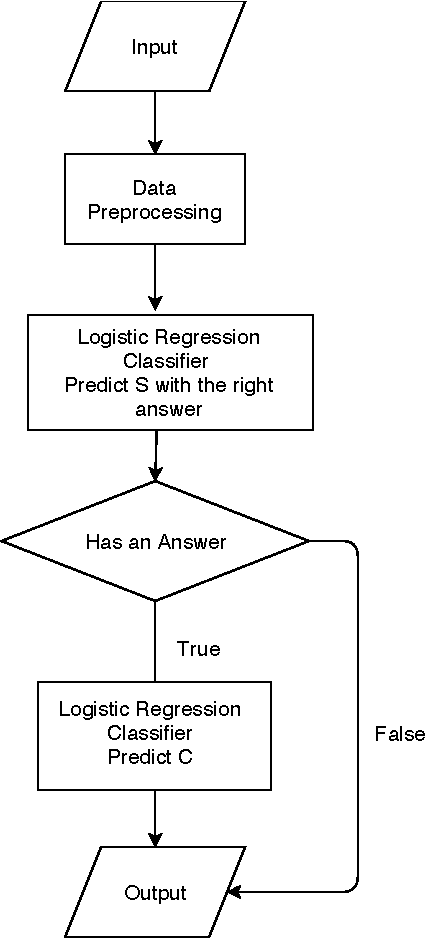
\includegraphics[scale=1]{../Figures/Flowchart.pdf}\centering
  \caption{Flowchart illustrating the two-stage classification approach}
  \label{arc-flowchart}
\end{figure}


\subsection{Feature Extraction} 
% In order for the classifier to find the sentence containing the answer, it must determine the sentence that is most similar to the question, and by similar we mean that a good candidate sentence  1) shares more words with the question. 2) has high cosine similarity with the question. 3) shares a syntactic similarity with the question. Thus, three main features have been selected to this end:
\begin{itemize}
\item \textbf{Cosine Similarity}: for every sentence in the paragraph as well as the question a word vector representation is created via InferSent (Conneau et al, 2017), which is a pre-trained sentence embeddings method that provides semantic representations for English sentences. InferSent is an encoder based on a bi-directional LSTM architecture with max pooling, trained on the Stanford Natural Language Inference (SNLI) dataset. Cosine distance score is calculated for each sentence-question pair. 
\item \textbf{Word Overlap}: calculates the Jaccard score between each sentence-question pair. Jaccard index is a method of computing the explicit similarity between two sets as follows: 
$$
J(Q,S) = \frac{|Q \cap S|}{|Q \cup S|}
$$
where Q and S are sets of words in question and sentence respectively.

\item \textbf{POS Overlap}: computes the Jaccard score over the part-of-speech-tag representation of sentences. In other words, instead of the word tokens, it checks similarity over POS tokens. We use the default POS-tagger in the SpaCy library of Python programming language to obtain the POS representation for the sentences and questions alike.
\end{itemize}
Using the three features above every question-sentence pair will have three scores and an additional binary feature indicating whether or not the question is answerable. 

\subsection{Training and Result} 
 We get the results shown in \ref{table:mlr-stage1}. Numbers in class column represents the index of the sentence in the paragraph containing the answer, and -1 indicates that the question has no answer in the paragraph. We also limit the number of sentences to 10. The results show that with simple features we get an F1 score of 0.71.

\begin{figure}
  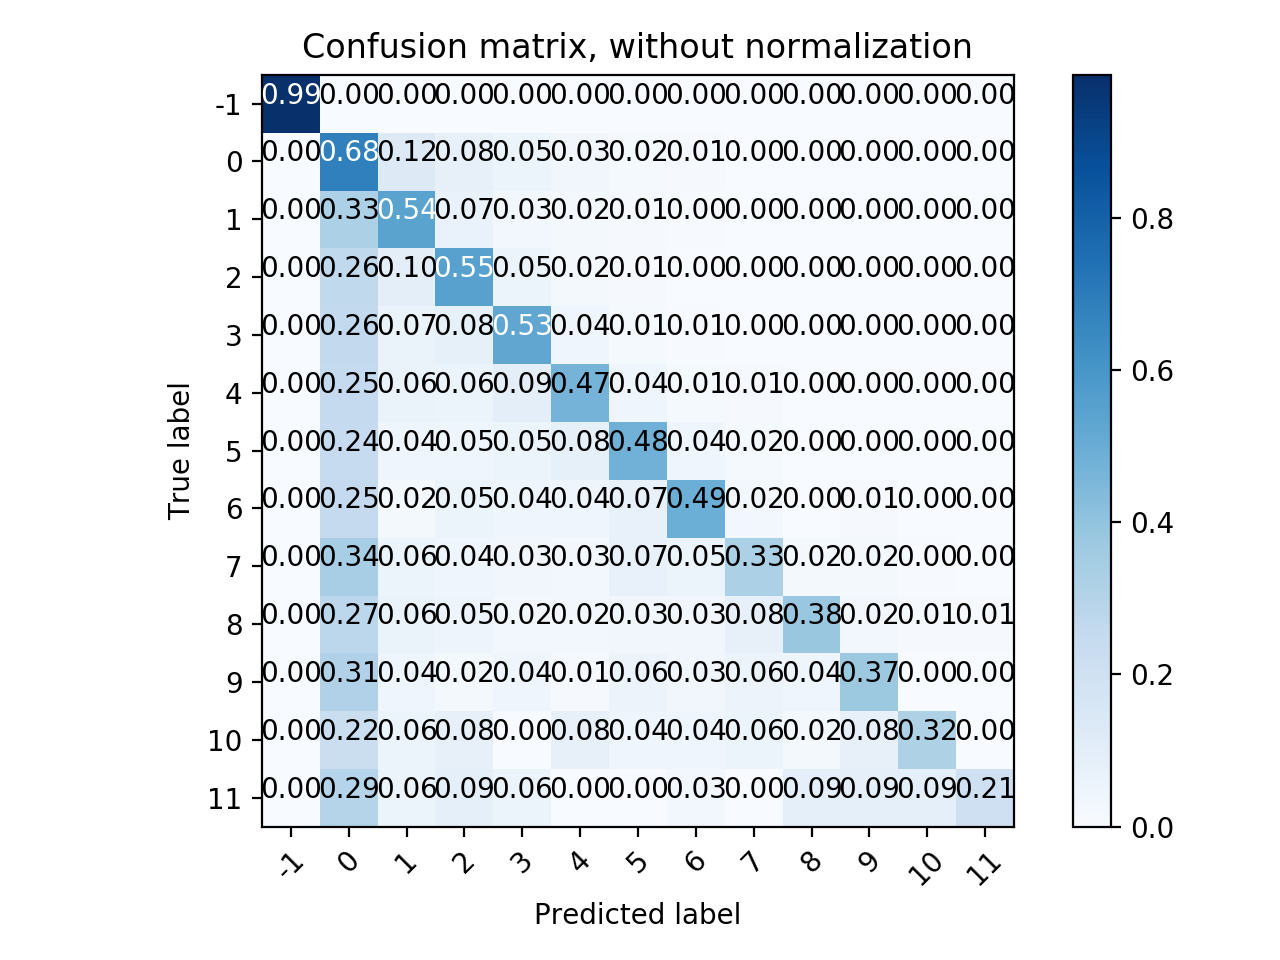
\includegraphics[scale=1]{Figure_1.png}\centering
  \caption{Confusion matrix shows which classes were predicted correctly}
\end{figure}

\begin{table}[]

\begin{tabular}{lllll}\centering
\hline \textbf{class} & \textbf{precision} & \textbf{recall} & \textbf{F1-score} \\ \hline

 -1    &    1    &    0.99    &    0.99        \\ 
0    &    0.47    &    0.68    &    0.56        \\
1    &    0.63    &    0.54    &    0.58    \\
2    &    0.62    &    0.55    &    0.58        \\
3    &    0.62    &    0.53    &    0.57        \\
4    &    0.58    &    0.47    &    0.52        \\
5    &    0.57    &    0.48    &    0.52        \\
6    &    0.57    &    0.49    &    0.53        \\
7    &    0.46    &    0.33    &    0.38    \\
8    &    0.56    &    0.38    &    0.45        \\
9    &    0.46    &    0.37    &    0.41        \\
10    &    0.48    &    0.32    &    0.39    \\
11    &    0.35    &    0.21    &    0.26        \\
\hline avg / total    &    0.72    &    0.71    &    0.71        \\ \hline

\end{tabular}
\caption{This table shows the results of running a multinomial regularized logistic regression. The class column represents the index of sentences within the paragraph, and -1 represents the unanswerable question case. Unpredicted classes are removed.}
\label{mlr-stage1}

\end{table}

\newpage

\section{Stage Two: Predicting the Answer Span}
\subsection{First Attempt}
To select the most plausible answer span from the candidate sentence, we design a number of features:
\begin{itemize}
\item \textbf{Constituents}: Using a constituency parser \citep{kitaev2018constituency}, we obtain all constituents in a candidate sentence. These constituents will be the classes from which we pick the right span.
\item \textbf{Contextual Overlap}: Constituents sharing context with the original question are potential candidates to be the correct answers. So we measure the cosine similarity between each constituent and the question:
$${ similarity } = \frac { \sum _ { i = 1 } ^ { n } C _ { |w| } Q _ { i } } { \sqrt { \sum _ { i = 1 } ^ { n } C _ { |w| } ^ { 2 } } \sqrt { \sum _ { i = 1 } ^ { n } Q _ { i } ^ { 2 } } }$$ 
where $w$ is the number of slide window around the candidate constituent. For our purposes features of size 2 and 3 are used. 

\item \textbf{Constituent Label}: Constituency parse tree label of the span combined with wh-word.
\end{itemize}
Out of 85K training example, the answer spans of nearly half of them are not within the constituents. However, answers can be part of the constituents.  For example, an answer span might be \textit{L'official} and the nearest constituent is \textit{L'official Magazine}. So for our first attempt, we remove all data points whose answers are not explicitly found within the constituents. This results in around 45K data point. Next, we train a logistic regression classifier with L2 regularization and 100 epochs, optimized by newton method 'newton-cg' on a MacBook Pro laptop with core i5 processor and 8 GB of RAM. Python modules used are Scikit-learn and SpaCy. The latter is used to drive the attentive-neural constituency parser (Kitaev, 2018). The result is 0.25 F1 score.




\subsection{Error Analysis of First Attempt}
%\subsection{Format of Electronic Manuscript}
%\label{sect:pdf}

\begin{figure}
  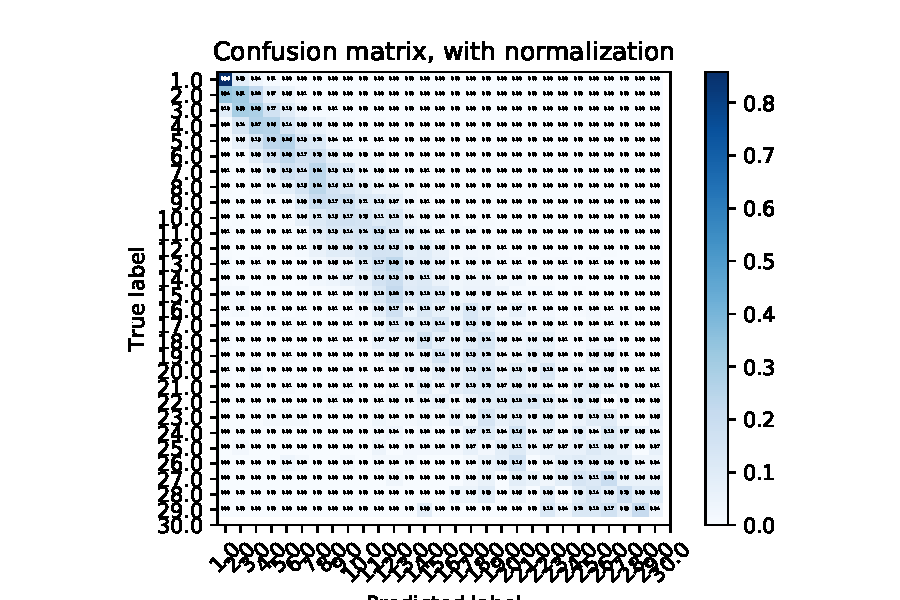
\includegraphics[scale=1]{../Figures/fig_iter1.pdf} \centering
  \caption{Confusion Matrix illustrating the first iteration of Stage2 LR. }
\end{figure} 



Looking at the confusion matrix, we notice that there is a data imbalance. Classes at the beginning have more supporting points, and therefore have less error than the others. However, class 2 has been identified as class 1 34\%. For example, the answer of \textit{At what age did Beyonce meet LaTavia Robertson?} is predicted as \textit{At age eight} while the correct answer is \textit{age eight}. Another example, the answer for \textit{How much was public expenditure on the island in 2001-2002?} is predicted to be \textit{Public expenditure} while the true answer is \textit{£10 million}. In this case, the phrase public expenditure appears in the question, which is a stronger candidate given the features designed.
Similarly, class 12 is predicted as class eleven 16\%. For example, the answer to the question \textit{Who supervised the design and implementation of the iPod user interface?} is \textit{Steve Jobs}, but it is predicted as \textit{Of Steve Jobs}. Another example, answer to \textit{What roles were women recruited for in the 1950s?} is \textit{in medicine, communication}, but it is predicted as \textit{logistics, and administration}. Given the features, we have designed it is very difficult for the classifier to recognize this settle difference between the classes. 


\subsection{Second Attempt}

In the first attempt, we have sacrificed valuable data because the answer span was not within the constituents of the candidate sentence. This time, we use all 85K, but we will face the same problem introduced in the previous section. The answer span can be a member of more than one constituent in the same sentence, and this will impose a very hard constraint on the performance because the inference can be close but not exact. Also because this problem requires more feature engineering efforts, we decided to leave it for future studies. Instead, we will set the target to the first constituent of which the span is a member. However, we will add three more features:

\begin{itemize}
\item \textbf{Distributional Distance}: We measure the distributional cosine similarity between the sum of all words in the contextual window and the question using Glove (Pennington, 2012). 

\item \textbf{Matching Word Frequencies}: Sum of the TF-IDF of the words that occur in both the question and the sentence containing the candidate answer.

\item \textbf{Lengths}: Number of words to the left and the right of the span.
\end{itemize}

For classification, we compare the performance of a logistic regression classifier with a similar configuration as the first stage to 3-layer feed-forward neural network of 128, 64 and 32 nodes respectively. The logistic regression achieves 0.35 F1 while the neural network does 0.42 F1 using Adam optimizer and 100 epochs. Looking at the confusion matrix, it is apparent that the new features (tf-idf and distributional cosine similarity) improve the performance. However, they could not recognize the settle difference among the phrase.  \\


\begin{figure}
  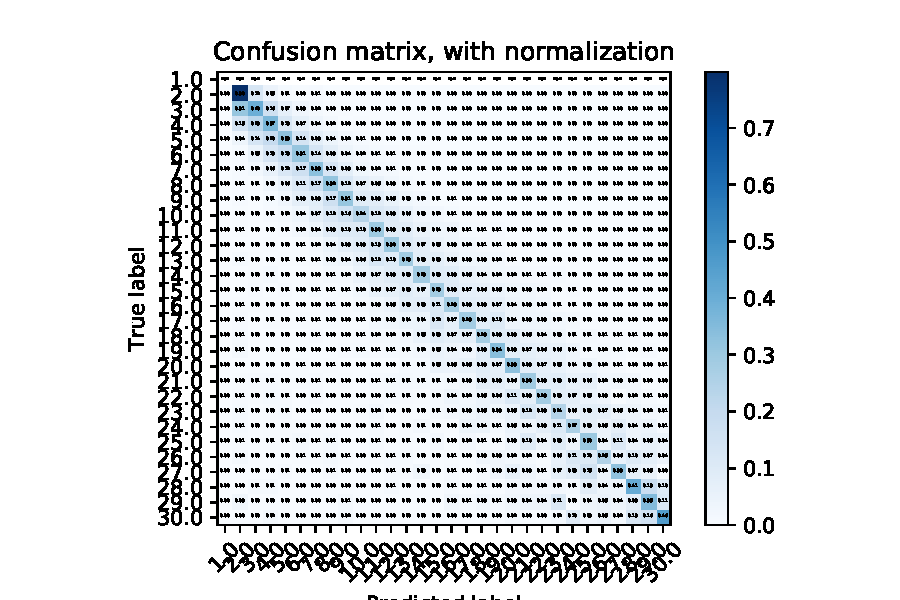
\includegraphics[scale=1]{../Figures/fig_1.pdf} 
  \caption{Confusion Matrix illustrating the Second iteration of Stage2 LR. }
\end{figure} 


\section{Conclusion}

We introduced a two-step classification method for automatic reading comprehension via SQUAD 2.0 dataset. Our stage1 classifier managed to find whether or not a question is answerable within a given passage and find the sentence containing the right answer with F1 score of 0.71. Our stage2 classifier manages to detect the exact span with F1 score of 0.35 even though the predicted answer is not distant from the exact answer. In order to improve the performance of our approach, future studies should investigate the usefulness of features generated from Named Entity Recognition, Semantic Role Labeling and Dependency Parsing processes, which are expected to be potential solutions to the problems we faced in this work. 